%\documentclass[PhD,two side]{srmuthesis}
%\documentclass[MS]{srmuthesis}
%\documentclass[MTech]{srmuthesis}
\documentclass[BTech]{srmuthesis}
\usepackage[dvipsnames]{xcolor}
\usepackage{times}
\usepackage{t1enc}
\usepackage{tikz}
\usepackage{subfigure}
\usepackage{pgfplots}
\usepackage{setspace} 
\usepackage{geometry}
\usepackage{graphicx}
\usepackage{epstopdf}
\usepackage{lscape}
\usepackage{fancyhdr}
\usepackage{natbib}
\usepackage{hyperref} % hyperlinks for references.
\usepackage{amsmath} % easier math formulae, align, subequations \ldots
\usepackage{amssymb}
\usepackage{wasysym}
\usepackage{titlesec}
\usepackage{textcomp}
\usepackage{pifont}
\usepackage{appendix} 
\usepackage{listings}
\usepackage{graphicx}
\usepackage{indentfirst}
\usepackage[section]{placeins}
\usetikzlibrary{decorations.pathmorphing}
\usetikzlibrary{shapes,arrows,shadows,patterns}
\usepackage[printonlyused]{acronym}
\usepackage{array}
\newcolumntype{L}{>{\centering\arraybackslash}m{4cm}}
\graphicspath{ {content/} }
\lstset{
basicstyle=\scriptsize\sffamily\color{black},
frame=single,
numbers=left,
numbersep=5pt,
numberstyle=\tiny\color{gray},
showspaces=false,
breaklines=true,
showstringspaces=false,
tabsize=1
}
\lstdefinelanguage{Kotlin}{
keywords={package, as, typealias, this, super, val, var, fun, for, null, true, false, is, in, throw, return, break, continue, object, if, try, else, while, do, when, yield, typeof, yield, typeof, class, interface, enum, object, override, public, private, get, set, import, abstract, },
keywordstyle=\color{NavyBlue}\bfseries,
ndkeywords={@Deprecated, Iterable, Int, Integer, Float, Double, String, Runnable, dynamic},
ndkeywordstyle=\color{BurntOrange}\bfseries,
emph={println, return@, forEach,},
emphstyle={\color{OrangeRed}},
identifierstyle=\color{black},
sensitive=true,
commentstyle=\color{gray}\ttfamily,
comment=[l]{//},
morecomment=[s]{/*}{*/},
stringstyle=\color{PineGreen}\bfseries\ttfamily,
morestring=[b]",
morestring=[s]{"""*}{*"""},
}
\definecolor{maroon}{rgb}{0.5,0,0}
\definecolor{darkgreen}{rgb}{0,0.5,0}
\lstdefinelanguage{XML}
{
basicstyle=\scriptsize\sffamily,
	morestring=[s]{"}{"},
	morecomment=[s]{?}{?},
	morecomment=[s]{!--}{--},
	commentstyle=\color{darkgreen},
	moredelim=[s][\color{black}]{>}{<},
	moredelim=[s][\color{red}]{\ }{=},
	stringstyle=\color{blue},
	identifierstyle=\color{maroon},
		morekeywords={
		android:background,
		android:clickable,
		android:contentDescription,
		android:iconifiedByDefault,
		android:id,
		android:layout_alignParentBottom,
		android:layout_alignParentRight,
		android:layout_height,
		android:layout_marginBottom,
		android:layout_marginLeft,
		android:layout_marginRight,
		android:layout_weight,
		android:layout_width,
		android:listSelector,
		android:orientation,
		android:paddingLeft,
		android:scaleType,
		android:src,
		android:text,
		android:textAppearance,
		android:textSize,
		android:textStyle,
		tools:context,
		xmlns:android,
		xmlns:tools,
	}
}



%\usepackage{nomencl}
%\newcommand{\bigsize}{\fontsize{16pt}{20pt}\selectfont}
%\renewcommand\nomname{\centerline {NOTATION}}
%\makenomenclature
\setcounter{MaxMatrixCols}{20}
\captionsetup[figure]{labelfont=bf}
\begin{document}
%%%%%%%%%%%%%%%%%%%%%%%%%%%%%%%%%%%%%%%%%%%%%%%%%%%%%%%%%%%%%%%%%%%%%%
% Title page

\title{An android application for different levels of college management} % Enter The Project Title

\firstauthor{ Vijay Krishna V }% Enter The Student name
\firstauthorregno{[Reg No: RA1511003020329]}
\secondauthor{ Chirag G Samtani }% Enter The Student name
\secondauthorregno{[Reg No: RA1511003020375]}
\thirdauthor{ Srushti Bompelli } % If there is no third author, leave the space blank like \thirdauthor{}
\thirdauthorregno{[Reg No: RA1511003020344]}
\fourthauthor{ Chaitanya Bachhav }
\fourthauthorregno{[Reg No: RA1511003020383]}
\guide{ Mr M. Prabu } % Enter your guide's name
\designation{ Asst. Professor } % Enter your guide's designation
\guidedepartment{Computer Science \& Engineering} % Enter the department name of your Guide 
\hod{Dr. JAGADEESAN,M.Tech.,Ph.D} % Enter HOD's name
\department{Computer Science \& Engineering} % Enter your department name
\date{OCT 2017} % Enter month and year of submission
%\nocite{*}

\maketitle
%%%%%%%%%%%%%%%%%%%%%%%%%%%%%%%%%%%%%%%%%%%%%%%%%%%%%%%%%%%%%%%%%%%%%%
%\vspace*{3in}
%\begin{center}
%{\Huge Dedicated to my Parents}
%\end{center}
%%%%%%%%%%%%%%%%%%%%%%%%%%%%%%%%%%%%%%%%%%%%%%%%%%%%%%%%%%%%%%%%%%%%%%
% Certificate
\certificate

%\vspace*{0.5in}



%%%%%%%%%%%%%%%%%%%%%%%%%%%%%%%%%%%%%%%%%%%%%%%%%%%%%%%%%%%%%%%%%%%%%%
% Abstract

\abstract
\begin{doublespacing}
\large\noindent Technical and scientific development has become one of the most essential changes in every aspect of the modern
day to make our work efficient and easier. The proposed
Android application has been designed to efficiently process the
management system of an institution at their different levels
of hierarchy, to reduce the physical work and confusion. Black
board is an application specifically for the faculty members and
the head of departments. The application will show required
content based on who is signing into the app. For instance, if
the dean logs into the app, he/she can view the details of all the
heads and their staff according to their departments, a HOD will
be able to see the details and availability of the faculty members
of their own department. The application will be able to display
most of the academic information like the timetables, availability
of the faculty, location of the classrooms etc. The database of the application can be modified and updated through a web portal
by a specific admin. Many future enhancements can be made to
the mobile application based on the institutions requirements.\\
\end{doublespacing}

\pagebreak
%%%%%%%%%%%%%%%%%%%%%%%%%%%%%%%%%%%%%%%%%%%%%%%%%%%%%%%%%%%%%%%%%%%%%%
% Acknowledgements
\acknowledgements
I would like to express my deepest gratitude to my guide, Mr. M. Prabu
his valuable guidance, consistent encouragement, personal caring, timely help and providing me with an excellent atmosphere for doing research. All through the work, in spite of his busy schedule, he has extended cheerful and cordial support to me for completing this project.\\



\begin{flushright}
{\bf Author}
\end{flushright}
%%%%%%%%%%%%%%%%%%%%%%%%%%%%%%%%%%%%%%%%%%%%%%%%%%%%%%%%%%%%%%%%%
% Table of contents etc.

\begin{singlespace}
\tableofcontents

\listoftables
\addcontentsline{toc}{chapter}{LIST OF TABLES}
\listoffigures
\addcontentsline{toc}{chapter}{LIST OF FIGURES}
\end{singlespace}


%%%%%%%%%%%%%%%%%%%%%%%%%%%%%%%%%%%%%%%%%%%%%%%%%%%%%%%%%%%%%%%%%%%%%%
\abbreviations
%\begin{acronym}[longest acronym must be entered here]
\begin{acronym}[OKID/ERA]

%\acro{acronym}{in detail}
\acro{API}{Application program interface}
\acro{HOD}{Head of department}
\acro{JSON}{Java Script Object Notation}
\acro{JVM}{Java Virtual Machine}
\acro{SQL}{Standardized Query Language}
\end{acronym}
% Use the syntax \ac{acronym} whereever you use this acronym.
% Abbreviations

%\noindent 
%\begin{tabbing}
%xxxxxxxxxxx \= xxxxxxxxxxxxxxxxxxxxxxxxxxxxxxxxxxxxxxxxxxxxxxxx \kill
%\textbf{TM}   \> Transfer Matrix \\
%\textbf{LMTM} \> Lumped Mass Transfer matrix \\
%\textbf{CMTM} \> Consistent Mass Transfer matrix \\
%\textbf{SCTM} \> Single Crack Transfer matrix \\
%\textbf{LCTM} \> Lumped Crack Transfer matrix \\
%\textbf{DCTM} \> Double Crack Transfer matrix \\
%\textbf{DOF} \> Degrees Of Freedom \\
%\textbf{GA} \> Genetic Algorithm  \\
%\textbf{PSO} \> Particle Swarm Optimization \\
%\textbf{SI} \> Structural Identification \\
%\end{tabbing}

\pagebreak

% The main text will follow from this point so set the page numbering
% to arabic from here on.
\pagenumbering{arabic}


%%%%%%%%%%%%%%%%%%%%%%%%%%%%%%%%%%%%%%%%%%%%%%%%%%
% Introduction.

%Enter your chapter number here
\chapter{Introduction}
\section{Overview}
The project is designed for the effective management of a college or an institution
according to their different levels of hierarchy present. In today's world it is very
important to work efficiently to avoid any confusion and for productive results. In the
administration of a college or an institution there exists various levels of hierarchy, the
responsibilities and functions differ at each level, in the existing system most of the work
done is paper work and it is manually carried out, this may lead to confusion and increase
of work load at each level. With increasing technology and tools in each and every aspect
of the world, it has become much easier and efficient to carry out any task. Our project
intends to give technical development to this particular field of college management. The
proposed android application will be able to store and retrieve the academic data and can
be accessed accordingly by the different levels of the management structure depending
upon their necessities and functionalities.

The project consists of an android application with a web portal and a common
database connecting them. The android application will have separate logins for the dean,
HOD, class in charge, faculty etc. once they login they will able to access the information required by them. For instance, if the dean logs into the app, he/she can view the details of all the heads and their staff according to their departments, a HOD will be able to see the details and availability of the faculty members of their own department and other information about their department. The main objective of the application is that all the academic information should be available at one place in an organized manner which can be easily accessible by just a click. The application helps in making tedious tasks like searching for classrooms or staff easier. The application also provides the facility to make calls to the required person from the app. Features like checking the availability of free staff helps in the effective management of time without free periods being wasted. The data in the application is stored in the database which will be updated from time to time. The application will be very user friendly to avoid any complications and it can be used by all the management members.

A web portal will be designed to update the database from time to time every year or every semester depending upon the college. It is easier to update the information than through the application itself. The web portal will consist of a login page through which the admin can login and update the information; the admin can be any faculty member with a secure login ID and password. The login details of the admin will be checked carefully and secure access will be given. Once the admin logs into the web portal he will be given access to update the all the information like changed time tables, details of the new students, change of classes etc. the website can be designed according to the convenience of the college, it will be user friendly with advanced features for the convenience of the user. The android application and the web portal are connected using a common database. The database contains all the information which is retrieved by the app and updated using the web portal. The data is stored in the database using a private cloud the information can only be accessed through secure login.

The scope and implementation of the project can be increased and developed with changing requirements. The project is designed and implemented using the latest and updated technologies for more efficiency and ease of access.
\section{Problem Statement}
Organized data is easier to work with than manual paper work, The problem in the existing system is that most of the work done by the management is paper work, there is no scope of organized data, each person have to maintain different files to access all the academic information. The main drawbacks of the existing college management system are:
\begin{itemize}
\item Manual work for all the teachers regarding attendance, updating and changing the attendance is difficult.
\item No way of knowing which teacher is free during which period.
\item No provision for rectification of mistakes.
\item Dean doesn't have access to everyone's contacts in one place.
\item Locating classes is not an easy task.
\item Contacting a higher official is difficult.
\end{itemize}
These drawbacks will be addressed by the project, the android application will facilitate the availability of all the information together, attendance can be updated through the app by the faculty whenever required; there will always be a way to rectify mistakes. The project will be implemented to address all the drawbacks of the existing system and improvise the effectiveness of the system.
\section{Objective}
The main objective of the proposed system is to introduce and implement technical advancement in the existing system of college management. The proposed the android application will be able to make the work easier by providing ease of access to the data required. Some of the main objectives of the project will be avoiding manual work for attendance, separate logins for different hierarchy of management, easier access to academic information, all information related to the particular person available in one application, effective management of time tables and free time, each level of management can access information relevant only to them (and not all information) through a secure login which keeps the data secured and avoids any misuse of data, increases overall efficiency of management. The web portal is used update the data in the database, one of the main objective of the web portal is to be user friendly to facilitate the admin to update the details with ease and the updated information should be secure which will be provide through secure login of the admin.
\section{Organization of the report}
There are five chapters in the report of the project android application for different levels of college management. The domain of the project is a common database connecting the android application and web portal. The report gives a comprehensible overview of the design and implementation details of the project, it helps understand the various technologies used in the project and the effective implementation of these technologies.
 
\subsection*{Chapter 1}
This chapter gives the basic introduction of the project, it gives the basic overview of the entire project and gives the details about the problem statement and the main objective of the project.

\subsection*{Chapter 2}
This chapter includes the literature survey which is a survey done on various base papers, it mainly gives the problems and conclusions for the domain of the project. The chapter also gives the description about  all the features of the existing system and its drawbacks and the proposed system and its advantages.

\subsection*{Chapter 3}
This chapter gives the requirements of the project in detail. It includes the basic purpose of the project, its scope, user requirements of the project. Software and Hardware specifications required by the project are given in detail in this chapter.

\subsection*{Chapter 4}
This chapter the complete information about the system design and the various modules present in the project. The chapter gives the system architecture and its description , it gives the detailed description about the data flow diagram. The module implementation is given in detail with the screen shots from the projects and the diagrams required. Data flow diagram and the process description for each module is separately given for better understanding.

\subsection*{Chapter 5}
This chapter deals with entire implementation of the system. The information about the platform of the project is given, the sample coding and the screen shots of the working model with proper description is given this chapter. The project will be done and the summary will be given.
\subsection*{Chapter 6}
The system implementation of the project will be given in this chapter. The project also gives an insight
about the implementation details,technologies used.
\subsection*{Chapter 7}
The conclusion of the project will be given in this chapter.The project also gives an insight about the future work which can be implemented through the project.

\chapter{Literature Survey}
\section{Introduction}
In this section we're going to talk about the various papers we have looked at which are related to our project.
\section{Existing System}
%TODO Autocite References Using BibLaTex
As mentioned in the paper 'Web Based Faculty Information Management System' by
S.R.Bharamagoudar, Geeta R.B., S.G.Totad (International Journal of Advanced Research in
Computer and Communication Engineering Vol. 2, Issue 6, June 2013) \cite{einstein}provides the system
using the web based technology, but it require the high speed internet connection which is a
further disadvantage of it. Instead of using the application provides the stand alone
environment so that can be easy to use on the slow internet connection also.. It can be easily
modified using the administration portal. If any requirement of the students or feedback can
also be taken using the application by individual student. It will also be easy for the teachers to
maintain their routine and make best use of the time which will help in advancement of
curriculum. The teaching plan is maintained and can be reported to the HOD of the
department. The app basically provides the platform for the teachers so that they can have
ease of their work as well as reducing the paper work will help to save the environment. This
application stated also provides standalone application platform to provide the various notices for the faculties.

Furthermore the paper 'Faculty Management System' by Shendkar Akshay, Lahor Ankit,
Kendre Anjali (International Journal of Advance Research and Innovative Ideas in
Education Volume-2, Issue-2, 2016).\cite{einstein1} The idea of the application is to allow the management
to interact and communicate with the faculty with ease. This can be done by means of using the internet connectivity for each and every staff-member. Thus the application can help the
faculty to manage and maintain the record digitally. All information fetched from the database server and maintained by administrator. The application has a section for login of Faculty. When the faculty logs in to the smartphone application then data fetches from the database and on faculty interface, similarly when admin logs in the portal he/she can edit the data.

Another such paper 'JIIT-Edu: An Android Application for College Faculty', by Upanya Singh,
Nadini Srivastava (Contemporary Computing (IC3), 2016 Ninth International Conference)  
aimed at minimizing the time consumption in tasks like taking attendance, pushing papers from
one level to another. The automated college management system was developed to increase
the productivity and technical growth of educational systems. The android app automates
certain tasks which when done manually take up a lot of time and energy. The app implements
Bluetooth and android technology for the making non-academic tasks paper-less and fast. The
app also improves student teacher interaction and communication via chat rooms. The app will
store profiles of every faculty member who can login through the interface. The app
implements Bluetooth to ensure each student is using their individual tag so as to prevent
proxies. The app also provides a platform for sharing study material. The user can download the material posted by other users.

Each of the above mentioned papers present systems which enable fast and paper-less
administration. These systems also provide a brilliant interface between user and data and
enable communication between users. These systems were developed with the aim of reducing manual work and enabling faster execution of necessary but non-academic activities. This project exhibits similar attributes and can be considered as a better and more reliable system as it overcomes the flaws present in the above systems as mentioned in the following pages.
\section{Issues in Existing System}
Now-a- days faculty deals with the papers and all the management regarding issue of making and
maintaining the all documents and records related the students and their daily conductance. It helps to
make sure that paper work is reduced to an efficient management model using the remote mobile
application.

\subsection{Web Based Faculty Information Management System}
The above system provides faculty information through a web application. There is no provision
of an interface for faculty through which they can login. Also this system consists of a
standalone website with no mobility at all. The site is not responsive which makes it
inaccessible for mobile devices like i-pad, smartphones, etc. Also there are no security
measures to ensure data privacy. The system doesn't implement login modules which kind of
makes it redundant and irregular since there is no separation between independent modules as
all the info is accessible to everyone due absence of abstraction.
\subsection{Faculty Management System}
This system consists of an android application which implements digital record maintenance.
The data-base is accessible through the app but making any changes to the stored data is
tedious as it involves editing the source-code of the application. This makes it difficult to edit
the database and thus the effectiveness of the system is in question. Also maintenance of the
data becomes tedious as admin user interface is not efficient. The system has unique login
credentials for every user but all the data present in the database is visible to everyone, some
part of this data may be irrelevant for certain users.
\subsection{JIIT- Edu: An Android App for college faculty}
Above system proposes an android application which provides a platform for faculty to share
study material, communicate and interact with other users through chat groups. The users can
upload and download documents through the chat groups, but there is no admin portal to
manage the application. There is no provision for handling direct access to database as the app
lacks implementation of hierarchical management.
\section{Summary of Literature Survey}
\subsection{Proposed system}
\subsubsection{Black-Board App}
This project consists of a web-portal and an android app for maintaining and accessing data. The web-
portal provides is an \ac{API} for managing the database, this portal can be accessed by the admin only
thereby ensuring data security. The admin privileges allow him/her to edit the data quite efficiently. The
data-entry can be commenced when an authorized login attempt is made to the admin app. The \ac{API} is
built using Django which is one the best frameworks that are available. The app will have login interface
through which the users can access data relevant to their tasks i.e. useless information will not be
visible, which is made possible by abstraction. Not all users can access every data, the access will be
restricted if the user does not login with proper credentials required. This will ensure data-security. The
HOD can view daily-schedules of every faculty who teaches in his/her department along with their
contact details. Dean login will allow access to details of all HOD’s and other relevant data. Once the app
makes a request the portal verifies the authentication details and sends data accordingly. The portal
interface allows for smooth transmission of data from data-base to the application. This overcomes the
problems mentioned in paper A \& paper B. Also the restricted access ensures privacy and is safer than
the system mentioned in paper C.
\chapter{Specifications}
\section{Introduction}
In this chapter, the specifications of this project are going to be discussed in detail. Topics like purpose, project scope and much more is also included.
\subsection{Purpose}
Teachers should do exactly what the name suggests, teach. The current education system does not allow them to do just that. Unfortunately, as the teachers have no other choice, they follow the system. Doing all the manual work of attendance and calculation of marks and all that itself takes up half their time. Valuable time that could have been spent on imparting knowledge to the students. This is where comes the purpose of our project. To decrease manual work for the teachers in colleges so that they can concentrate on imparting their knowledge to students.
\subsection{Project Scope}
The scope of this project is huge. We plan to first implement this only in our college but as soon as that happens, we plan to approach various colleges where this problem of manual work persists and implement it there. After colleges, we can move on to schools and other institutions. The scope is endless.  
\section{Overall Description}
In overall description we're going to discuss about how the project is implemented. Description of what was done, the features, the user characteristics, operating environment, implementation constraints and much more.
\subsection{Product Features}
The various feature in our application and web interface will include the following:
\begin{itemize}
\item Separate logins for different hierarchy of management.
\item Easier access to academic information.
\item All information related to the particular person available in one application.
\item Effective management of timetables.
\item Each level of management can access information relevant only to them (and not all information).
\item Increases overall efficiency of management.
\item Locations of classes in the campus can be found in the application.
\item Academic information of all the students can be found under the separate class teacher's login.
\item The dean can access the contact information of every teacher on the campus.
\item The dean can call any teacher he wishes to from the application itself.
\item The \ac{HOD} of each department can view the performance of students of his/ her department.
\item Free periods of teachers can be seen through the application which will help in allocating them to classes where teachers are absent.
\end{itemize}
\subsection{User classes and characteristics}
The various user classes and their characteristics are given below:

\subsubsection{Login}
The login class takes the login information from the user and authenticates it. If the information matches with that of the database, it directs it to another page based on whether the user is a teacher, dean or a HOD of a department.                          
\subsubsection{Menu}
The menu is where the user can select what functionality he/she wants to use. The various menu items include:
\begin{itemize}
\item Class time tables
\item Teacher time tables
\item Available Staff
\item Class Location
\end{itemize}

\subsubsection{Class Time Tables}
This is where the user can select the particular class he/she wants the time table to and can view the time table of the same in the application itself.
\subsubsection{Available Staff}
This is where the senior staff can view the free periods of the teachers so that he/she can assign the teacher another class in case there is a class without a teacher at that point.
\subsubsection{Class Location}
This is where the user can enter the class he/she wants to go to and the result will be the location of the class in the campus. We later plan to add a student login where this feature will also be available.
\subsubsection{Call Staff}
This is where the dean will be able to browse through all the teachers and HODs and will be able to call any one of them from the application itself.
\subsubsection{Teacher Time Tables}
This is where the HOD can select the teacher from his/her department and view the time table of the same in the application itself.
\subsection{Operating environment}
The Android SDK includes a virtual mobile device emulator that runs on your computer. The
emulator lets you prototype, develop and test Android applications without using a physical
device. The Android Emulator simulates a device and displays it on your development computer.
It lets you prototype, develop, and test Android apps without using a hardware device. You can
launch an app on the emulator when you run your project, or you can drag an APK file onto the
emulator to install it. As with a hardware device, after you install an app on a virtual device, it
remains until you uninstall or replace it. If needed, you can test how multiple apps, such as your
own or system apps, work with each other. You interact with the emulator just as you would with
a hardware device, but using your mouse and keyboard, and emulator buttons and controls. The
emulator supports virtual hardware buttons and touchscreens, including two-finger operations, as
well as directional pads (D-pads), trackballs, wheels, and various sensors. You can dynamically
resize the emulator window as needed, zoom in and out, change the orientation, and even take a
screenshot.

When your app is running on the emulator, it can use the services of the Android platform to
invoke other apps, access the network, play audio and video, accept audio input, store and
retrieve data, notify the user, and render graphical transitions and themes. The emulator has
controls that let you easily send incoming phone calls and text messages, specify the location of
the device, simulate fingerprint scans, specify network speed and status, and simulate battery
properties. The emulator can simulate an SD card and internal data storage; you can drag a file,
such as a graphics or data file, onto the emulator to store it.
\subsection{Design and Implementation Constraints, Assumptions and dependencies}
The one dependency that this project has is that the data has to be fed into the web portal every semester and this responsibility has to be taken up by one individual.

\paragraph{Material Design} is a design language developed by Google. Material design is a comprehensive guide for visual, motion, and interaction design across platforms and devices. A single underlying system that allows for a unified experience across platforms and device sizes.
\section{External Interface Requirements}
In this part, we're going to discuss about the external interface requirements like the user interface, hardware and software interface:
\subsection{User Interface}
We've used xml for making the user interface of the android application. And HTML, CSS for the user interface of the web portal. This is a very important part of the project as without a proper UI, the user wouldn't be able to navigate through the application properly and in the end, that is of no use.
\subsection{Hardware Interface}
There is no physical database where all the data is stored, it's all stored in the cloud. The other physical component required will be the smartphone itself which every user will undoubtedly have.
\subsection{Software Interface}
The various components of the software interface are given below:
\subsubsection{Login Interface}
The login class takes the login information from the user and authenticates it. If the information matches with that of the database, it directs it to another page based on whether the user is a teacher, dean or a HOD of a department.                          
\subsubsection{Menu Interface}
The menu is where the user can select what functionality he/she wants to use. The various menu items include:
\begin{itemize}
\item Class time tables
\item Teacher time tables
\item Available Staff
\item Class Location
\end{itemize}

\subsubsection{Class Time Tables Interface}
This is where the user can select the particular class he/she wants the time table to and can view the time table of the same in the application itself.
\subsubsection{Available Staff Interface}
This is where the senior staff can view the free periods of the teachers so that he/she can assign the teacher another class in case there is a class without a teacher at that point.
\subsubsection{Class Location Interface}
This is where the user can enter the class he/she wants to go to and the result will be the location of the class in the campus. We later plan to add a student login where this feature will also be available.
\subsubsection{Call Staff Interface}
This is where the dean will be able to browse through all the teachers and HODs and will be able to call any one of them from the application itself.
\subsubsection{Teacher Time Tables Interface}
This is where the HOD can select the teacher from his/her department and view the time table of the same in the application itself.
\subsection{Communication Interface}
There are three levels of communications happening at a given moment in the app's lifecycle. They are mentioned below:
\begin{itemize}
\item Web-portal to database
\item Database to web-portal
\item Application to database
\end{itemize}
Note that the web-portal and the application do not communicate at all. The data is fed through the web portal and is stored in the database which is then accessed by the application to display it to the users. 
\section{Other non-functional Requirements}
In this section, we're going to discuss about the other non-functional requirements like performance and security requirements. 
\subsection{Performance Requirements}
Other than a smartphone and an internet connection, nothing will be required to run this application with the highest performance.
\subsection{Security Requirement}
The app automatically encrypts the password of the user and hence the passwords are kept safe. In case the user forgets his/ her password, extra steps will be taken to make sure that the user is identified first. And hence, security is taken care of.
\chapter{System Design}
\section{Introduction}
This chapter gives detailed information about the system design of the project, system design includes the requirements of the system, the entire flow of the process of the system. Understanding the design of the system helps in the better implementation of the system. This chapter includes the system architecture, in the system architecture the relationship and the process flow among the components is given. The data flow diagram gives the detailed process flow between the various modules of the system; a module is a separate unit of software or hardware. Typical characteristics of modular components include portability, which allows them to be used in a variety of systems, and interoperability, which allows them to function with the components of other systems. The  software and hardware requirements includes all data, functional and behavioral requirements of the software under production or development it also includes the hardware specifications required by the project. The software and hardware requirements of the system help in analyzing the basic architecture of the system. 

The architecture diagram for the project android application for different levels of college management gives the basic process flow between the android and the web portal and some of the modules. The data flow diagram includes the process between the modules like login page, time table display page etc.
\section{System Architecture}
The architecture of a system is a model to describe or analyze a system. The system architecture basically consists various structures present in them and the relationship between them. The design and architecture of the system can be represented and modeled using an architecture diagram and the data flow diagram. The architecture diagram will consist of  basic components and modules. The data flow diagram describes about every module and the process flow, the pictorial representation of these helps in analyzing the design of the system.
\begin{figure}[htbp]
	\centering
	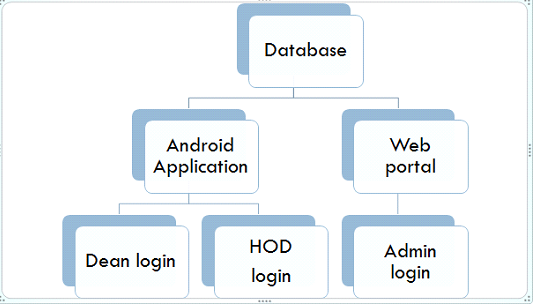
\includegraphics[width=\linewidth, height=7cm,keepaspectratio]{arch}
	\caption{System Architecture}
	\label{fig:arch}
\end{figure}
\begin{figure}[htbp]
	\centering
	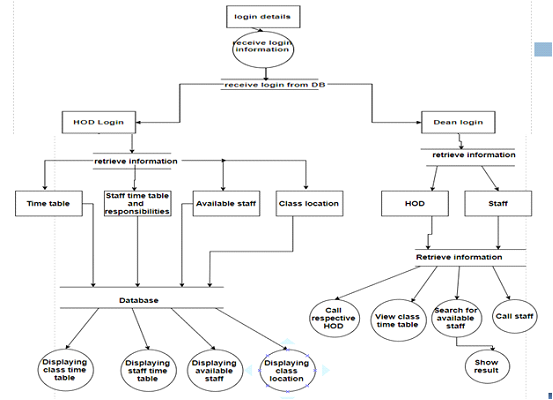
\includegraphics[width=\linewidth, height=7cm,keepaspectratio]{dataflow}
	\caption{DataFlow Diagram}
	\label{fig:data}
\end{figure}
\section{Description}
The architecture diagram includes the main components the android application, database and the web portal. The diagram shows that the database is the back end of the system, it connects the android application and the web portal, the data updated through the web portal is retrieved by the database and accessed by the android application. 
The dean login, the HOD login and the admin login are the main modules of the system. Through a secure login the user will be able to access the functionalities of these modules. 

In the data flow diagram the various modules and the process flow between these modules is comprehensibly described.
The symbols used in the data flow diagram are described in the below figure:
\begin{figure}[htbp]
	\centering
	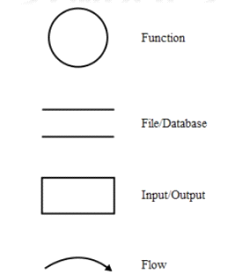
\includegraphics[width=\linewidth, height=7cm,keepaspectratio]{desc}
	\caption{Symbold used in the DataFlow Diagram}
	\label{fig:sym}
\end{figure}
The data flow diagram shows the step by step process of the android application. First there will be a login page to take the input login of the user, once the user enters the login information the data will be retrieved by the database and acted upon. The next functional page depending on the login will be shown, if it is a HOD login options like time table, available staff, staff time tables and responsibilities, location of the classes will be given, the user has to choose one and the given input will be retrieved by the database and the respective information like displaying the location of the class which has been entered, displaying the information about available staff etc. can be accessed or viewed. If it is a dean login options like HOD or staff will be given, once the input is received by the database the next respective module like displaying the details of the HOD of a particular department, contacting a HOD, checking for staff etc. will be accessed.
\section{System Requirements}
\subsection{Software specifications}
The software specifications required to build the software of the system are:\\
Android Studio\\
Django framework\\
python\\
JDK\\
web browser\\
GIT 
\subsection{Hardware specifications}
The hardware specifications required by the system are:\\
Dual-core 64-bit processor\\
8 GB of memory\\
Up to 24 GB of internal storage\\
4-4 GB RAM\\
Hard disk capacity 40GB
\section{Summary}
Thus the system design has been analyzed and a detailed description about the design of this system has been given in this chapter. The analysis of the design of the system gives the detailed overview about the project, in this chapter detailed description of each and every module is given which briefs the user about the various features and advantages of the project. This chapter has also given information about the available features and options in the project. The requirements of the system also have been given for the better understanding of the technology used in the project.

\chapter{Module Description}
\section{Introduction}
In this section, we're going to talk about the various modules in this project. We have divided the whole project into many sub sections and the three main modules of the project will be discussed below. Apart from discussing about it, the work flow diagram of each module is going to be provided to provide a clear idea of what the module is going to be and in-turn how the whole project is going to be.
\section{Login Module}
\begin{figure}[htbp]
	\centering
	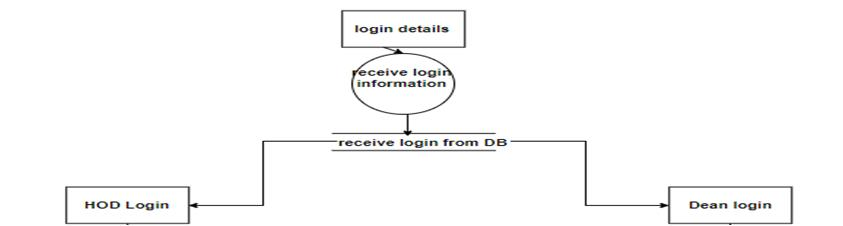
\includegraphics[width=\linewidth, height=7cm,keepaspectratio]{loginmodule}
	\caption{Work flow diagram for Login Module}
	\label{fig:loginmodule}
\end{figure} 
\paragraph{Description}
The log in is the most important part of the application as it segregates the teachers from the deans and hods and provides a layer of security to the app. The user will enter the email and password and based on the suffix of the email, the app will first authenticate the user and then redirect to the main teacher or hod activity.
\section{HOD Module}
\begin{figure}[htbp]
	\centering
	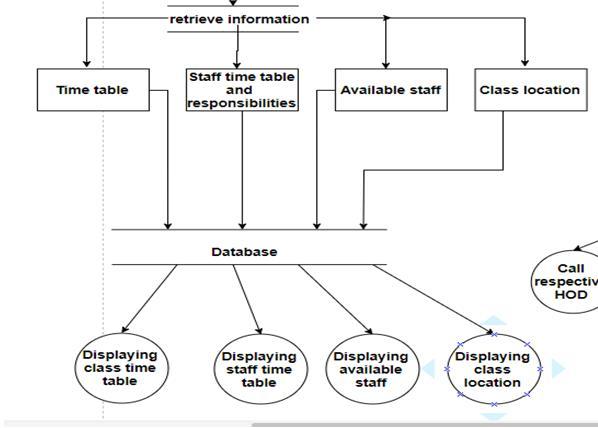
\includegraphics[width=\linewidth, height=7cm,keepaspectratio]{hodmodule}
	\caption{Work flow diagram for HOD Module}
	\label{fig:hodmodule}
\end{figure} 
\paragraph{Description}
This is the HOD module where all the information that the HOD of each department of the college can view is here. The various sub modules include:
\begin{itemize}
\item Class Location
\item Available Staff
\item Staff Time Tables
\item Class Time Tables
\end{itemize}
All this information is stored in the database and is accessed only once and will be stored offline so that the HODs can view the information without internet too.
\section{Dean Module}
\begin{figure}[htbp]
	\centering
	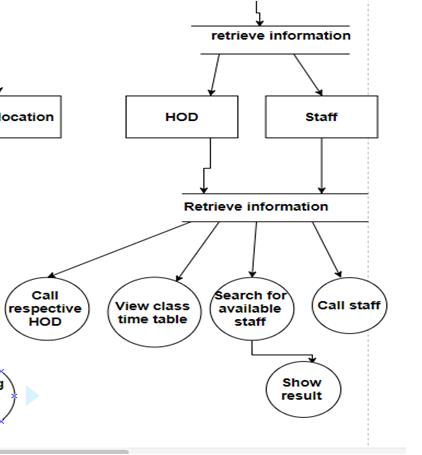
\includegraphics[width=\linewidth, height=7cm,keepaspectratio]{deanmodule}
	\caption{Work flow diagram for Dean Module}
	\label{fig:deanmodule}
\end{figure} 
\paragraph{Description}
This is the Dean module where all the information that the Dean of the college can view is here. The various sub modules include:
\begin{itemize}
\item Head of Departments
\item Staff
\end{itemize}
All this information is stored in the database and is accessed only once and will be stored offline so that the Dean can view the information without internet too.
\section{Summary}
As has been shown above, the project has been divided into 3 major modules and they have been explained in detail. The login module being the one that handles the security and the other two modules are the ones that display information to the dean and HODs.
\chapter{System Implementation}
\section{Overview of the Platform}
\subsection{Java}
The Java language is a key pillar in Android, an open source mobile operating system. Although Android, built on the Linux kernel, is written largely in C, the Android SDK uses the Java language as the basis for Android applications.

Java is a general-purpose computer programming language that is concurrent, class-based, object-oriented, and specifically designed to have as few implementation dependencies as possible. It is intended to let application developers "write once, run anywhere" (WORA), meaning that compiled Java code can run on all platforms that support Java without the need for recompilation. Java applications are typically compiled to bytecode that can run on any Java virtual machine (\ac{JVM}) regardless of computer architecture. 
\subsection{Kotlin}
Kotlin is a Concise, Simple,Safe and Statically typed programming language focused on Interoperability with Java. 

One can Avoid entire classes of errors such as null pointer exceptions. Improves code readability as it Drastically reduces the amount of boilerplate code. While the syntax is not compatible with Java, Kotlin is reliant on Java code from the existing Java Class Library, such as the collections framework. 
Kotlin is a fully supported programming language on Android.
\subsection{Django(Web Framework)}
Django is a free and open-source web framework, written in Python, which follows the model-view-template (MVT) architectural pattern.

Django's primary goal is to ease the creation of complex, database-driven websites. Django emphasizes reusability and "pluggability" of components, rapid development, and the principle of don't repeat yourself. Python is used throughout, even for settings files and data models. Django also provides an optional administrative create, read, update and delete interface that is generated dynamically through introspection and configured via admin models.
\subsection{Git}
Git is a version control system for tracking changes in computer files and coordinating work on those files among multiple people. It is primarily used for source code management in software development, but it can be used to keep track of changes in any set of files. As a distributed revision control system it is aimed at speed, data integrity, and support for distributed, non-linear workflows.
\subsection{RESTful \ac{API}}
Representational state transfer (REST) or RESTful web services is a way of providing interoperability between computer systems on the Internet. REST-compliant Web services allow requesting systems to access and manipulate textual representations of Web resources using a uniform and predefined set of stateless operations.

An \ac{API} for a website is code that allows two software programs to communicate with each another.A RESTful \ac{API} explicitly takes advantage of HTTP methodologies. They use GET to retrieve a resource; PUT to change the state of or update a resource, which can be an object, file or block; POST to create that resource; and DELETE to remove it.
\subsection{\ac{JSON}}
JavaScript Object Notation or \ac{JSON} is an open-standard file format that uses human-readable text to transmit data objects consisting of attribute-value pairs and array data types (or any other serializable value). It is a very common data format used for asynchronous browser-server communication.

JSON is built on two structures:
A collection of name/value pairs. In various languages, this is realized as an object, record, struct, dictionary, hash table, keyed list, or associative array.
An ordered list of values. In most languages, this is realized as an array, vector, list, or sequence.
\subsection{Android}
Android is a mobile operating system developed by Google, based on the Linux kernel and designed primarily for touchscreen mobile devices such as smartphones and tablets.

Android's user interface is mainly based on direct manipulation, using touch gestures that loosely correspond to real-world actions, such as swiping, tapping and pinching, to manipulate on-screen objects, along with a virtual keyboard for text input. 
\subsection{Android Studio}
The Official IDE for Android. Android Studio provides the fastest tools for building apps on every type of Android device.

World-class code editing, debugging, performance tooling, a flexible build system, and an instant build/deploy system all allow you to focus on building unique and high quality apps.
\subsection{SQLite}
SQLite is an in-process library that implements a self-contained, serverless, zero-configuration, transactional \ac{SQL} database engine. The code for SQLite is in the public domain and is thus free for use for any purpose, commercial or private.

SQLite is an embedded \ac{SQL} database engine. Unlike most other \ac{SQL} databases, SQLite does not have a separate server process.SQLite is a compact library. With all features enabled, the library size can be less than 500KiB. SQLite a popular database engine choice on memory constrained gadgets such as cellphones, PDAs, and MP3 players. Performance is usually quite good even in low-memory environments.

\subsection{Open Source Libraries for Android}
\paragraph{Glide}
Glide is a fast and efficient open source media management and image loading framework for Android that wraps media decoding, memory and disk caching, and resource pooling into a simple and easy to use interface.
\paragraph{Retrofit}
A type-safe HTTP client for Android and Java.
This library provides a powerful framework for authenticating and interacting with \ac{API}s and sending network requests with OkHttp network.
This library makes downloading JSON or XML data from a web \ac{API} fairly straightforward. Once the data is downloaded then it is parsed into a Plain Old Java Object (POJO).
\paragraph{Stetho}
Stetho is a sophisticated debug bridge for Android applications developed by facebook. When enabled, developers have access to the Chrome Developer Tools feature natively part of the Chrome desktop browser.
Network inspection is possible with the full spectrum of Chrome Developer Tools features, including image preview, JSON response helpers.
SQLite databases can be visualized and interactively explored with full read/write capabilities.
\paragraph{ProGuard}
ProGuard is the most popular optimizer for Java bytecode. It makes your Java and Android applications up to 90\% smaller and up to 20\% faster. ProGuard also provides minimal protection against reverse engineering by obfuscating the names of classes, fields and methods.
\section{Implementation Details}

\subsection{Simulation Parameters}
The Android SDK includes a virtual mobile device emulator that runs on your computer. The emulator lets you prototype, develop and test Android applications without using a physical device.
\subsubsection{Unit Testing}
This is the first level of testing. In this different modules are tested against the specifications produced during the design of the module. During this testing the number of the arguments is compared to input parameters, matching of parameter and arguments etc. All five modules are checked separately, each test case is given to each unit and it is checked. The result is checked to see if the actual outcome is same as the expected outcome.A unit test is also called a module test because it tests the individual units of code that comprise the application. Each test validates a single module that was built to perform a certain task with the expectation that it will behave in a specific way. During this testing the number of the arguments is compared to input parameters, matching of parameter and arguments etc. All five modules are checked separately, each test case is given to each unit and it is checked. The result is checked to see if the actual outcome is same as the expected outcome.A unit test is also called a module test because it tests the individual units of code that comprise the application. Each test validates a single module that was built to perform a certain task with the expectation that it will behave in a specific way.
\subsubsection{Integration testing}
Integration testing is a process where all the separate modules are combined together
and its working is checked. There are two approaches to this : bottom-up and top-down
integration.At first the branch, semester and grade selection modules are integrated and checked.Top-down approach is being used in this software testing.
\subsubsection{User acceptance testing}
User acceptance of a system is the factor for the success of any system. The system
under consideration is tested for the user acceptance by constantly keeping in touch
with the prospective system user at the time of developing wherever required.
\begin{itemize}
\item Input screen design.
\item Output screen design.
\item Online message to guide the user.
\item Format of the reports and other outputs
\end{itemize}
\subsubsection{Functional Testing}
Functional testing ensures that the application is working as per the requirements. Most of the test conducted for this is driven by the user interface and call flow
\subsubsection{Performance Testing}
This testing process is undertaken to check the performance and behavior of the application under certain conditions such as low battery, bad network coverage, low available memory, simultaneous access to application’s server by several users and other conditions. Performance of an application can be affected from two sides:application’s server side and client’s side. Performance testing is carried out to check both.
\subsubsection{Memory Leakage Testing}
Memory leakage happens when a computer program or application is unable to manage the memory it is allocated resulting in poor performance of the application and the overall slowdown of the system. As mobile devices have significant constraints of available memory, memory leakage testing is crucial for the proper functioning of an application
\subsubsection{Interrupt Testing}
 An application while functioning may face several interruptions like incoming calls or network coverage outage and recovery. The different types of interruptions are:
\begin{itemize}
\item Incoming and Outgoing SMS and MMS
\item Incoming and Outgoing calls
\item Incoming Notifications
\item Battery Removal
\item Cable Insertion and Removal for data transfer
\item Network outage and recovery
\item Media Player on/off
\end{itemize}
An application should be able to handle these interruptions by going into a suspended state and resuming afterwards.
\subsubsection{Usability testing}
Usability testing is carried out to verify if the application is achieving its goals and getting a favorable response from users. This is important as the usability of an application is its key to commercial success (it is nothing but user friendliness).Another important part of usability testing is to make sure that the user experience is uniform across all devices.This section of testing hopes to address the key challenges of the variety of mobile devices and the diversity in mobile platforms/OS, which is also called device fragmentation. One key portion of this type of usability testing is to be sure that there are no major errors in the functionality, placement, or sizing of the user interface on different devices.
\subsubsection{Installation testing}
Certain mobile applications come pre-installed on the device whereas others have to be installed from the store. Installation testing verifies that the installation process goes smoothly without the user having to face any difficulty. This testing process covers installation, updating and uninstalling of an application
\subsubsection{Security Testing}
Security Testing: To check for vulnerabilities to hacking, authentication and authorization policies, data security, session management and other security standards.
\subsubsection{Results}
\begin{table}[htbp]
	\centering
\begin{tabular}{|L|L|L|c|}

	\hline
	Testing Parameters & Expected Output  & Actual Output &Result\\
	\hline
		\hline
	Authentication & Authenticate user by validating credentials from \ac{API} & User is Authenticated &Pass\\
		\hline
	Fetch Faculty Timetable & Fetch faculty time-table from the \ac{API} & Time-table fetched and stored locally &Pass\\
		\hline
	Fetch Class Timetable & Fetch class time-table from the \ac{API} & Time-table fetched and stored locally &Pass\\
		\hline
	Fetch Class Location &  Fetch class location from the \ac{API} & class location displayed & Pass\\
		\hline
	Check Faculty Availability & fetch available faculty from the database & displayed available faculty &Pass\\
		\hline
	Admin Portal Authentication & Authenticate Admin &Credentials Validated &Pass\\
		\hline
	Admin Portal-Update/modify Database   & Changes should reflect in the app & Data Changed &Pass\\
	\hline
\end{tabular}
\caption{Test-Cases}
\label{tab:test-cases}
  \end{table}
\begin{table}[htbp]
	\centering
\begin{tabular}{|c|L|c|}
	\hline
	Name of Test & \ac{API} Level & Test Result\\
	\hline
		\hline
	Unit testing & Lollipop , Nougat & Pass\\
		\hline
	Integration testing & Lollipop , Nougat & Pass\\
		\hline
	User Acceptance testing & Lollipop , Nougat & Pass\\
		\hline
	Functional testing & Lollipop , Nougat & Pass\\
		\hline
	Usability testing & KitKat , Nougat & Pass \\
		\hline
	Memory Leakage testing & Marshmellow , Nougat & Pass\\
		\hline
	Performance testing   & KitKat , Nougat & Pass\\
		\hline
	Interrupt testing & Marshmellow , Nougat & Pass\\
		\hline
	Installation tests & Lollipop , Nougat & Pass\\
		\hline
	Security Testing & Lollipop , Nougat & Pass\\
	
	\hline
\end{tabular}
\caption{Test-Results}
\label{tab:test-results}
\end{table}

\subsection{Sample coding}
\begin{lstlisting}[language=Kotlin,caption={Retrofit Interface}, label={lst:retrofit}]
package com.notadeveloper.app.blackboard

import com.facebook.stetho.okhttp3.StethoInterceptor
import io.reactivex.Observable
import okhttp3.OkHttpClient
import retrofit2.Retrofit
import retrofit2.adapter.rxjava2.RxJava2CallAdapterFactory
import retrofit2.converter.moshi.MoshiConverterFactory
import retrofit2.http.Field
import retrofit2.http.FormUrlEncoded
import retrofit2.http.POST

interface RetrofitInterface {
@FormUrlEncoded
@POST("login")
fun authUser(@Field("user") user: String, @Field("pass") pass: String): Observable<Faculty>

@FormUrlEncoded
@POST("getfacultytimetable")
fun getfacultytimetable(@Field("user") user: String, @Field("pass") pass: String, @Field("id") id: String): Observable<timetable>

@FormUrlEncoded
@POST("getclasstimetable")
fun getclasstimetable(@Field("user") user: String, @Field("pass") pass: String, @Field("class") class: String): Observable<timetable>

@FormUrlEncoded
@POST("getavailablestaff")
fun getavailablestaff(@Field("user") user: String, @Field("pass") pass: String, @Field("day") day: String, @Field("hour") hour: String): Observable<List<String>>

companion object Factory {
fun create(): RetrofitInterface {
val retrofit = Retrofit.Builder()
.addCallAdapterFactory(RxJava2CallAdapterFactory.create())
.addConverterFactory(MoshiConverterFactory.create().asLenient())
.client(OkHttpClient.Builder().addNetworkInterceptor(StethoInterceptor()).build())
.baseUrl("http://blackboard.xyz/")
.build()
}
}
}
\end{lstlisting}
\begin{lstlisting}[language=XML,caption={Faculty Dashboard}, label={lst:faculty-dashboard}]
<?xml version="1.0" encoding="utf-8"?>
<RelativeLayout xmlns:android="http://schemas.android.com/apk/res/android"
xmlns:app="http://schemas.android.com/apk/res-auto"
xmlns:tools="http://schemas.android.com/tools"
android:id="@+id/activity_main"
android:layout_width="match_parent"
android:layout_height="match_parent"
android:paddingBottom="@dimen/activity_vertical_margin"
android:paddingLeft="@dimen/activity_horizontal_margin"
android:paddingRight="@dimen/activity_horizontal_margin"
android:paddingTop="@dimen/activity_vertical_margin"
tools:context="com.example.lenovo.bb.HodActivity">

<Button
android:text="Available staff"
android:layout_width="match_parent"
android:layout_height="wrap_content"
android:layout_below="@+id/button"
android:theme="@style/button"
android:id="@+id/button2" />

<Button
android:text="class location"
android:layout_width="match_parent"
android:layout_height="wrap_content"
android:layout_below="@+id/button2"
android:theme="@style/button"
android:id="@+id/button3"
/>

<Button
android:text="class time table"
android:layout_width="match_parent"
android:layout_height="wrap_content"
android:id="@+id/button4"
android:layout_below="@+id/imageView2"
android:theme="@style/button"
android:layout_centerHorizontal="true"
/>

<ImageView
android:layout_width="wrap_content"
android:layout_height="wrap_content"
android:src="@drawable/blckbrdcover"
android:id="@+id/imageView2"
android:adjustViewBounds="true"
android:scaleType="fitXY"
android:layout_alignParentTop="true"
android:layout_alignParentLeft="true"
/>

<Button
android:text="Staff time table and responsibilities"
android:layout_width="match_parent"
android:layout_height="wrap_content"
android:id="@+id/button"
android:theme="@style/button"
android:layout_below="@+id/button4"
android:layout_alignParentLeft="true"
android:layout_alignParentStart="true" />
</RelativeLayout>
\end{lstlisting}
\subsection{Screen Shots}
\subsubsection{Faculty Login (fig\ref{fig:faculty-login})}
Every faculty whomsoever install the
application will have to provide its email-id, password and
phone number during its one time registration process. These
informations are first matched with the online database and then
stored in mobile database.
\begin{figure}[htbp]
	\centering
	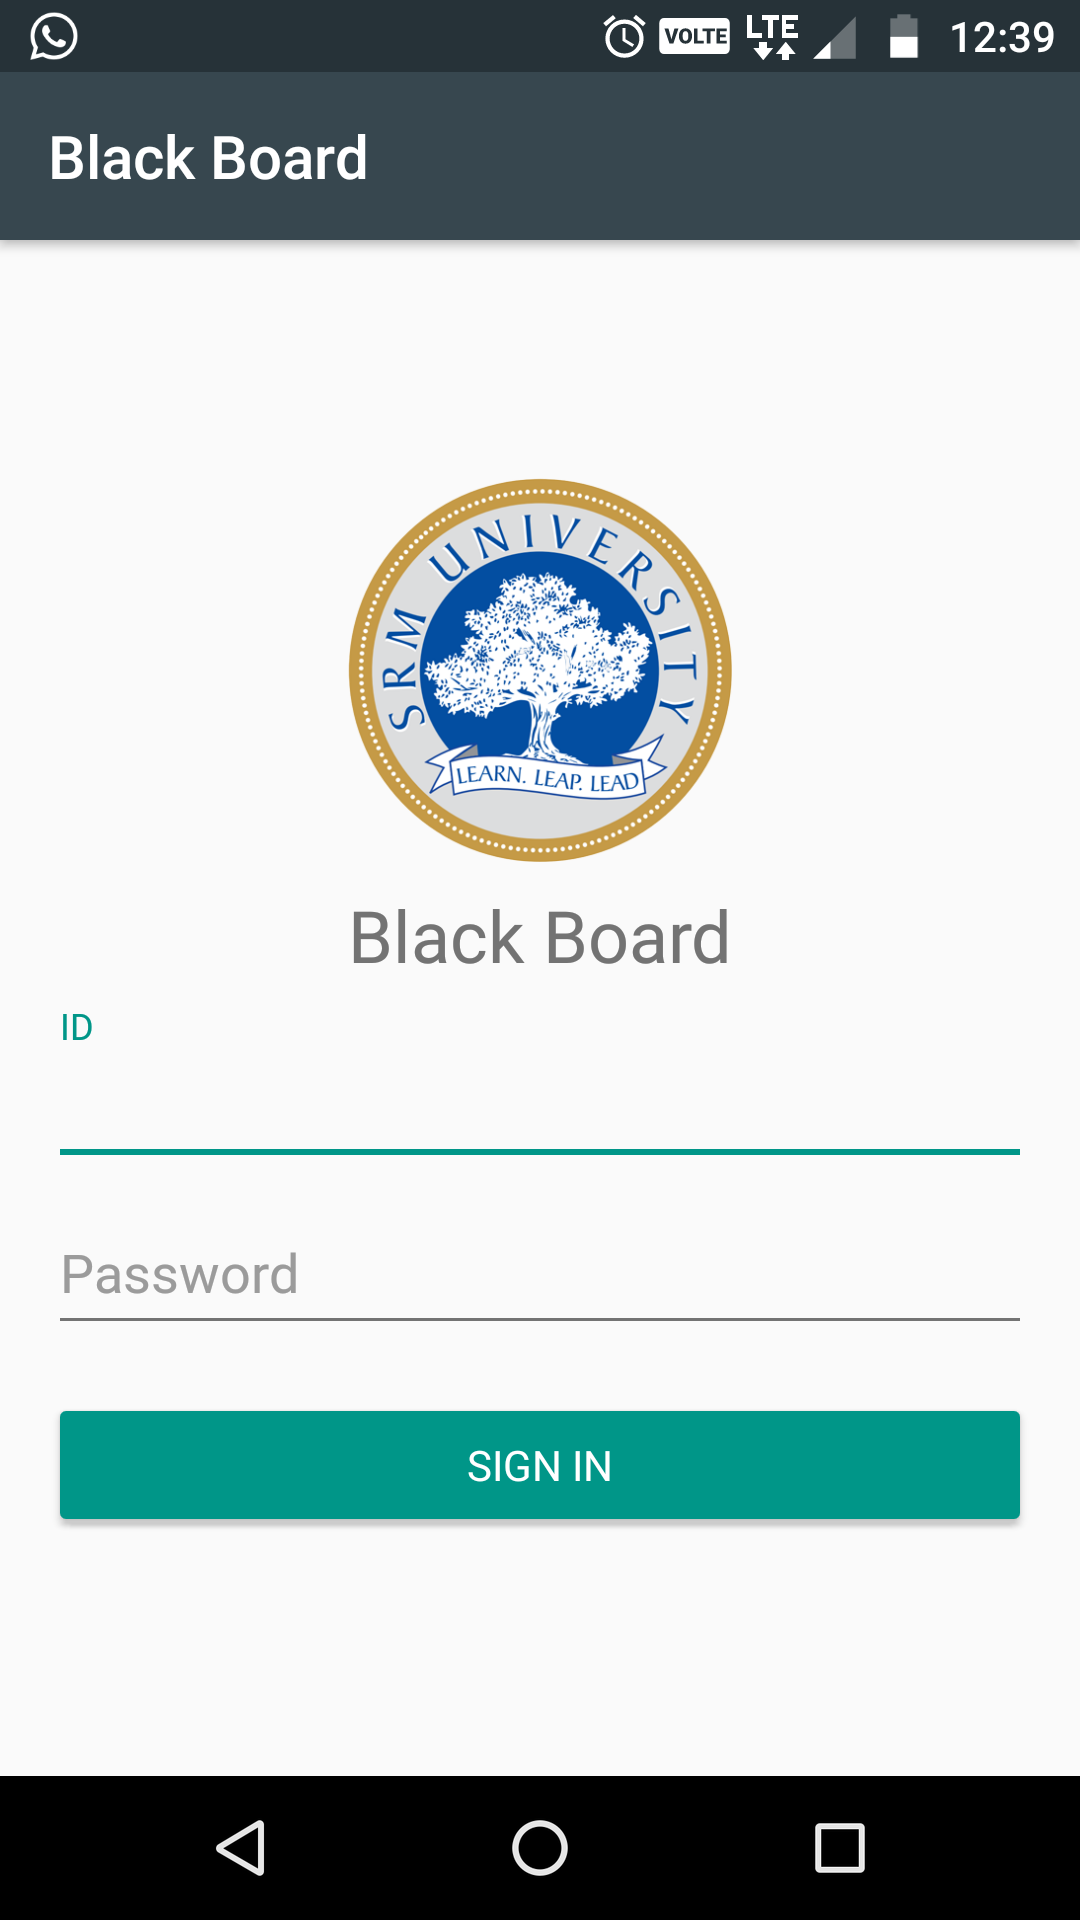
\includegraphics[width=\linewidth, height=7cm,keepaspectratio]{login}
	\caption{Faculty Login}
	\label{fig:faculty-login}
\end{figure}
\subsubsection{Faculty Dashboard (fig\ref{fig:faculty-dashboard})}
All information related to the particular person
available in one application. Faculty can check his/her timetable, class location, class timetable with the click of a button.
\begin{figure}[htbp]
	\centering
	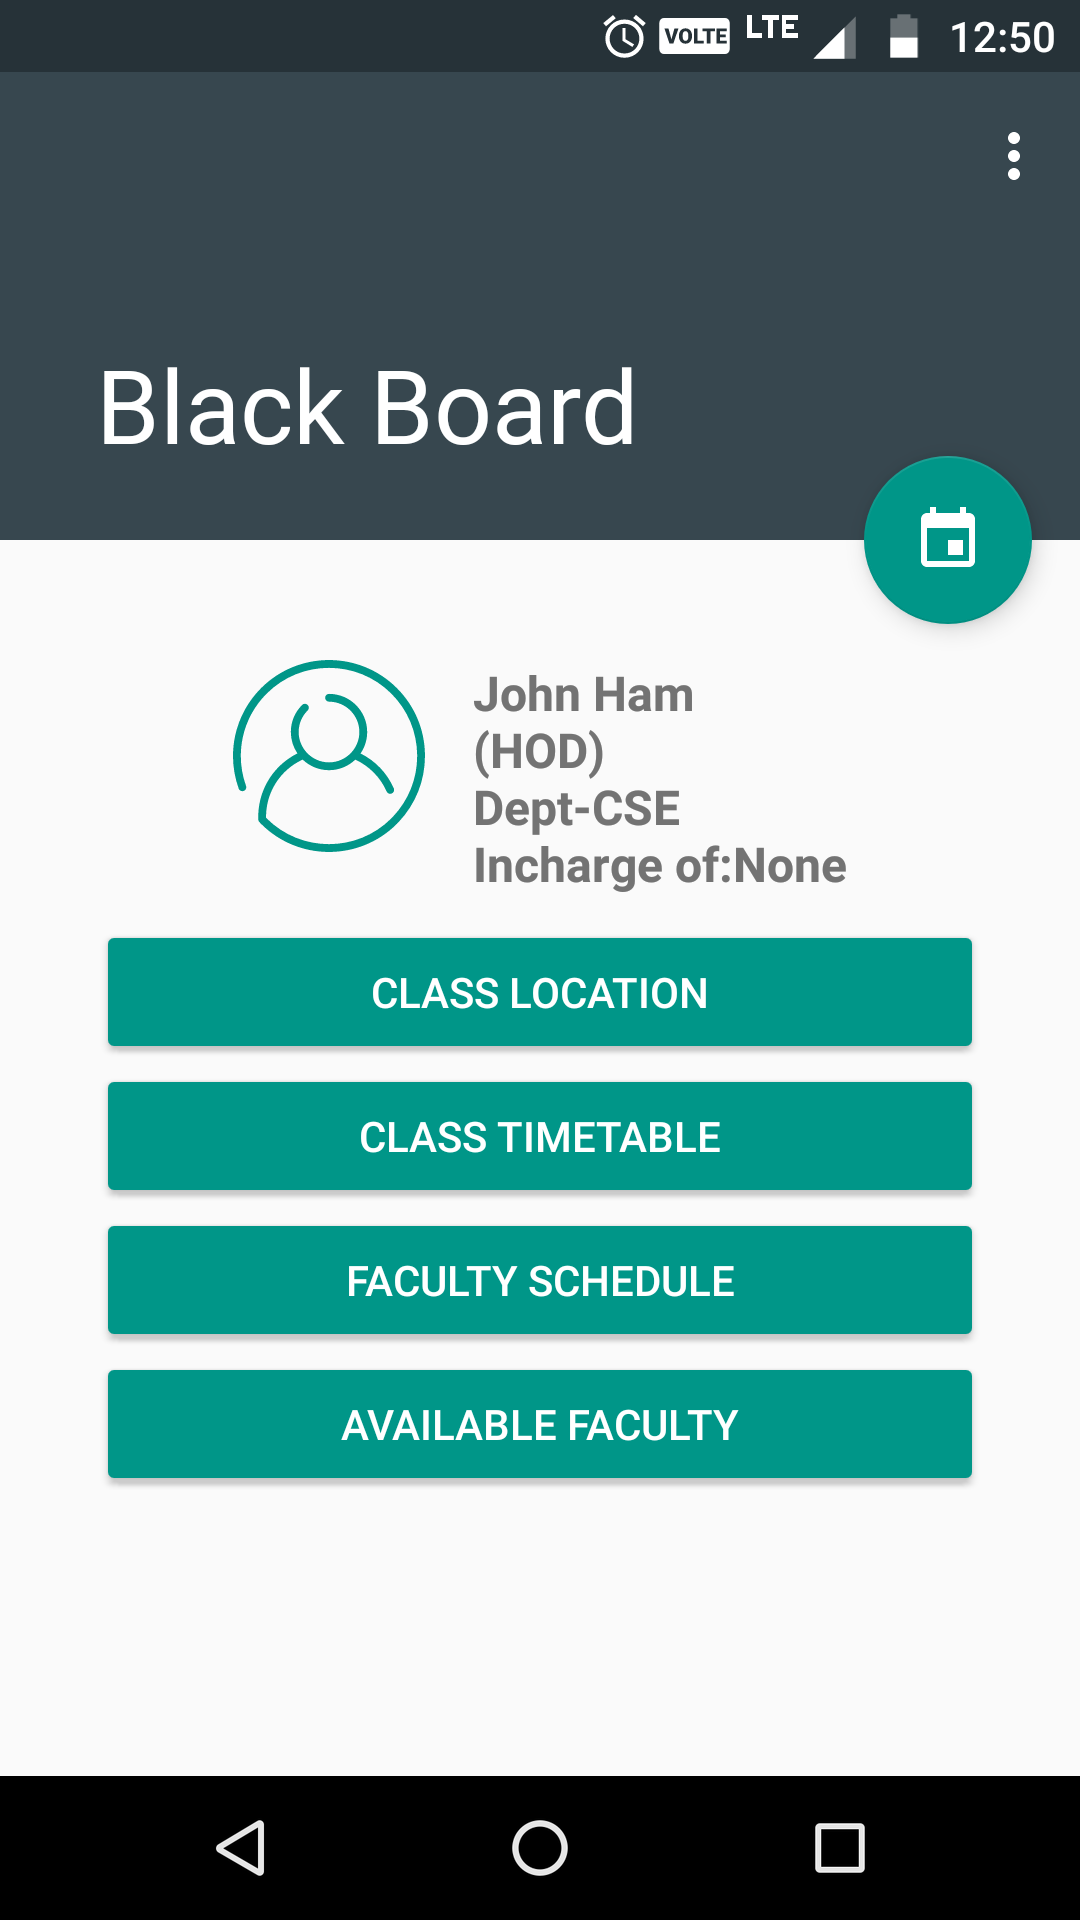
\includegraphics[width=\linewidth, height=7cm,keepaspectratio]{dashboard}
\caption{Faculty Dashboard}
\label{fig:faculty-dashboard}
\end{figure} 
\subsubsection{Check available faculty (fig\ref{fig:available-faculty})}
Hod can easily check the available faculty by selecting the day and hour.
\begin{figure}[htbp]
	\centering
	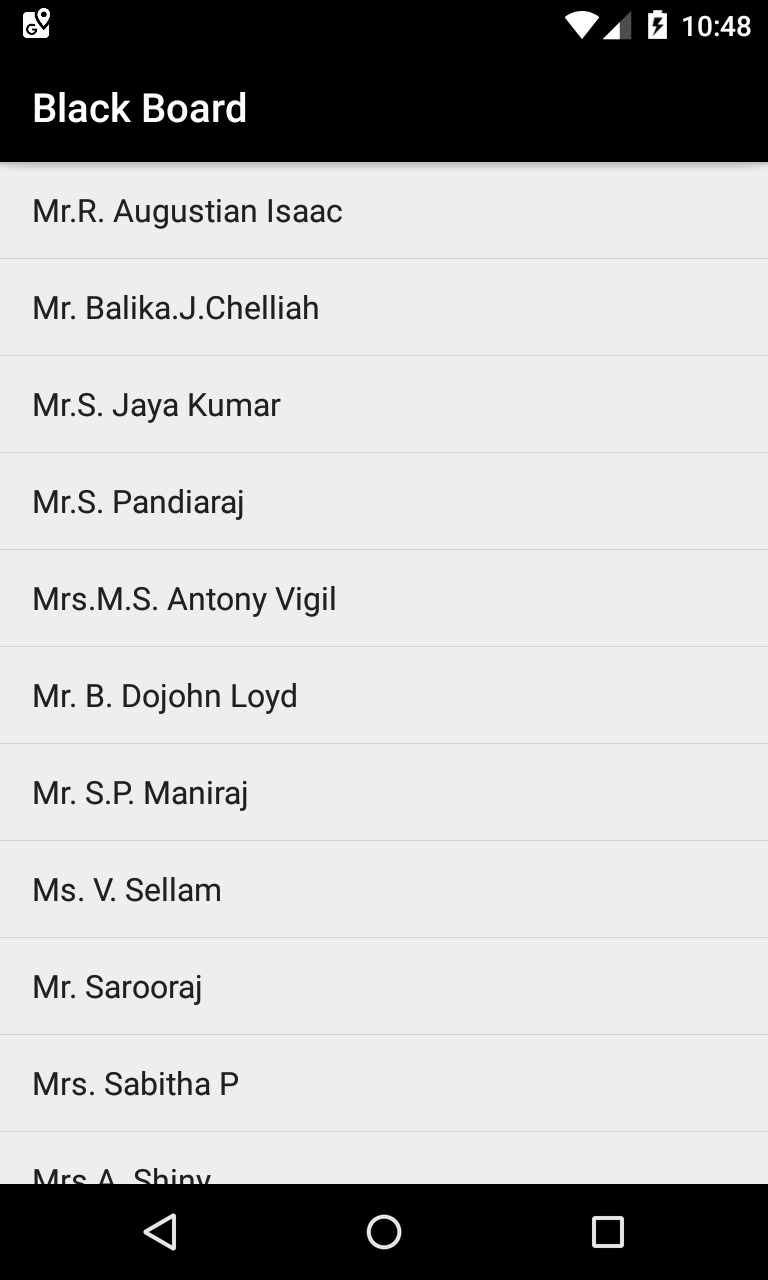
\includegraphics[width=\linewidth, height=7cm,keepaspectratio]{checkavailability}
\caption{Check Available Faculty}
\label{fig:available-faculty}
\end{figure} 
\subsubsection{Faculty Timetable (fig\ref{fig:faculty-timetable})}
The Hod can check the timetable of a particular faculty by querying the database.
\begin{figure}[htbp]
	\centering
	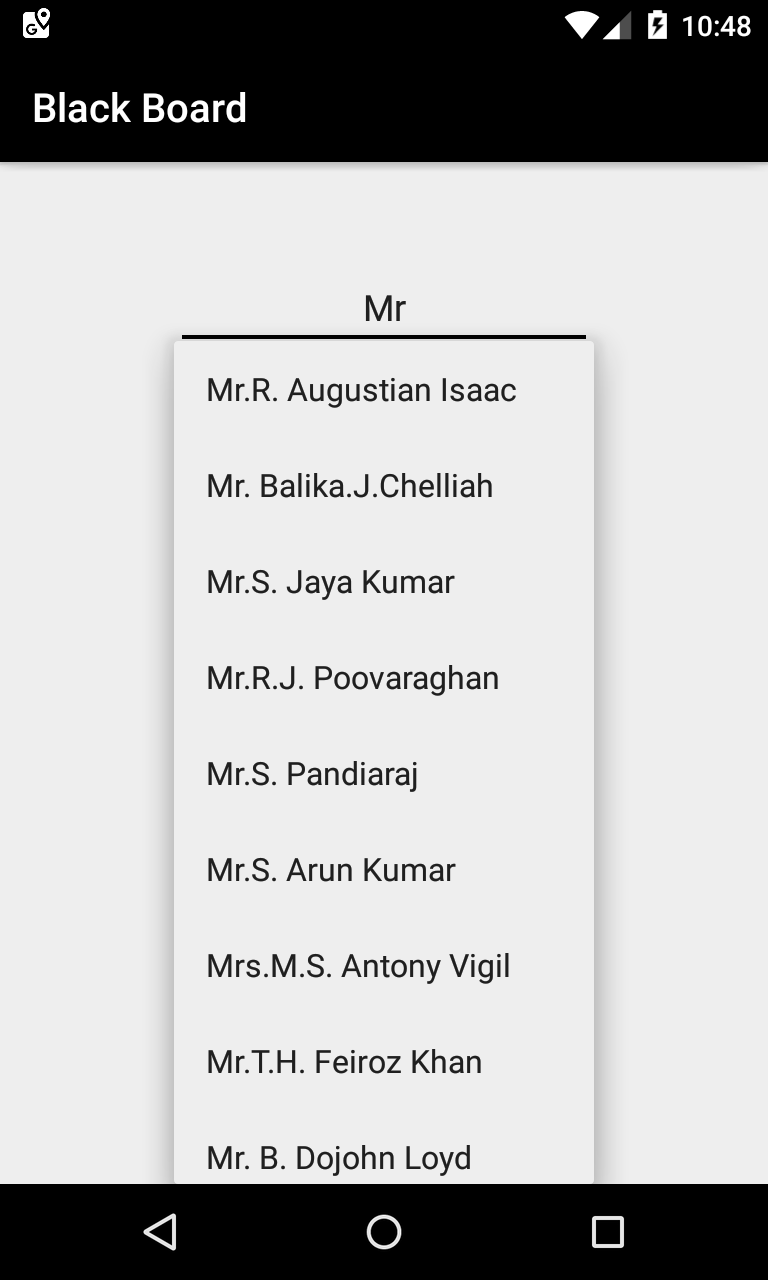
\includegraphics[width=\linewidth, height=7cm,keepaspectratio]{facultytimetable}
\caption{Faculty Timetable}
\label{fig:faculty-timetable}
\end{figure}
\subsubsection{Check Class Timetable (fig\ref{fig:class-timetable})}
The faculty can check the timetable of a particular class by selecting the year, section of the class.
\begin{figure}[htbp]
	\centering
	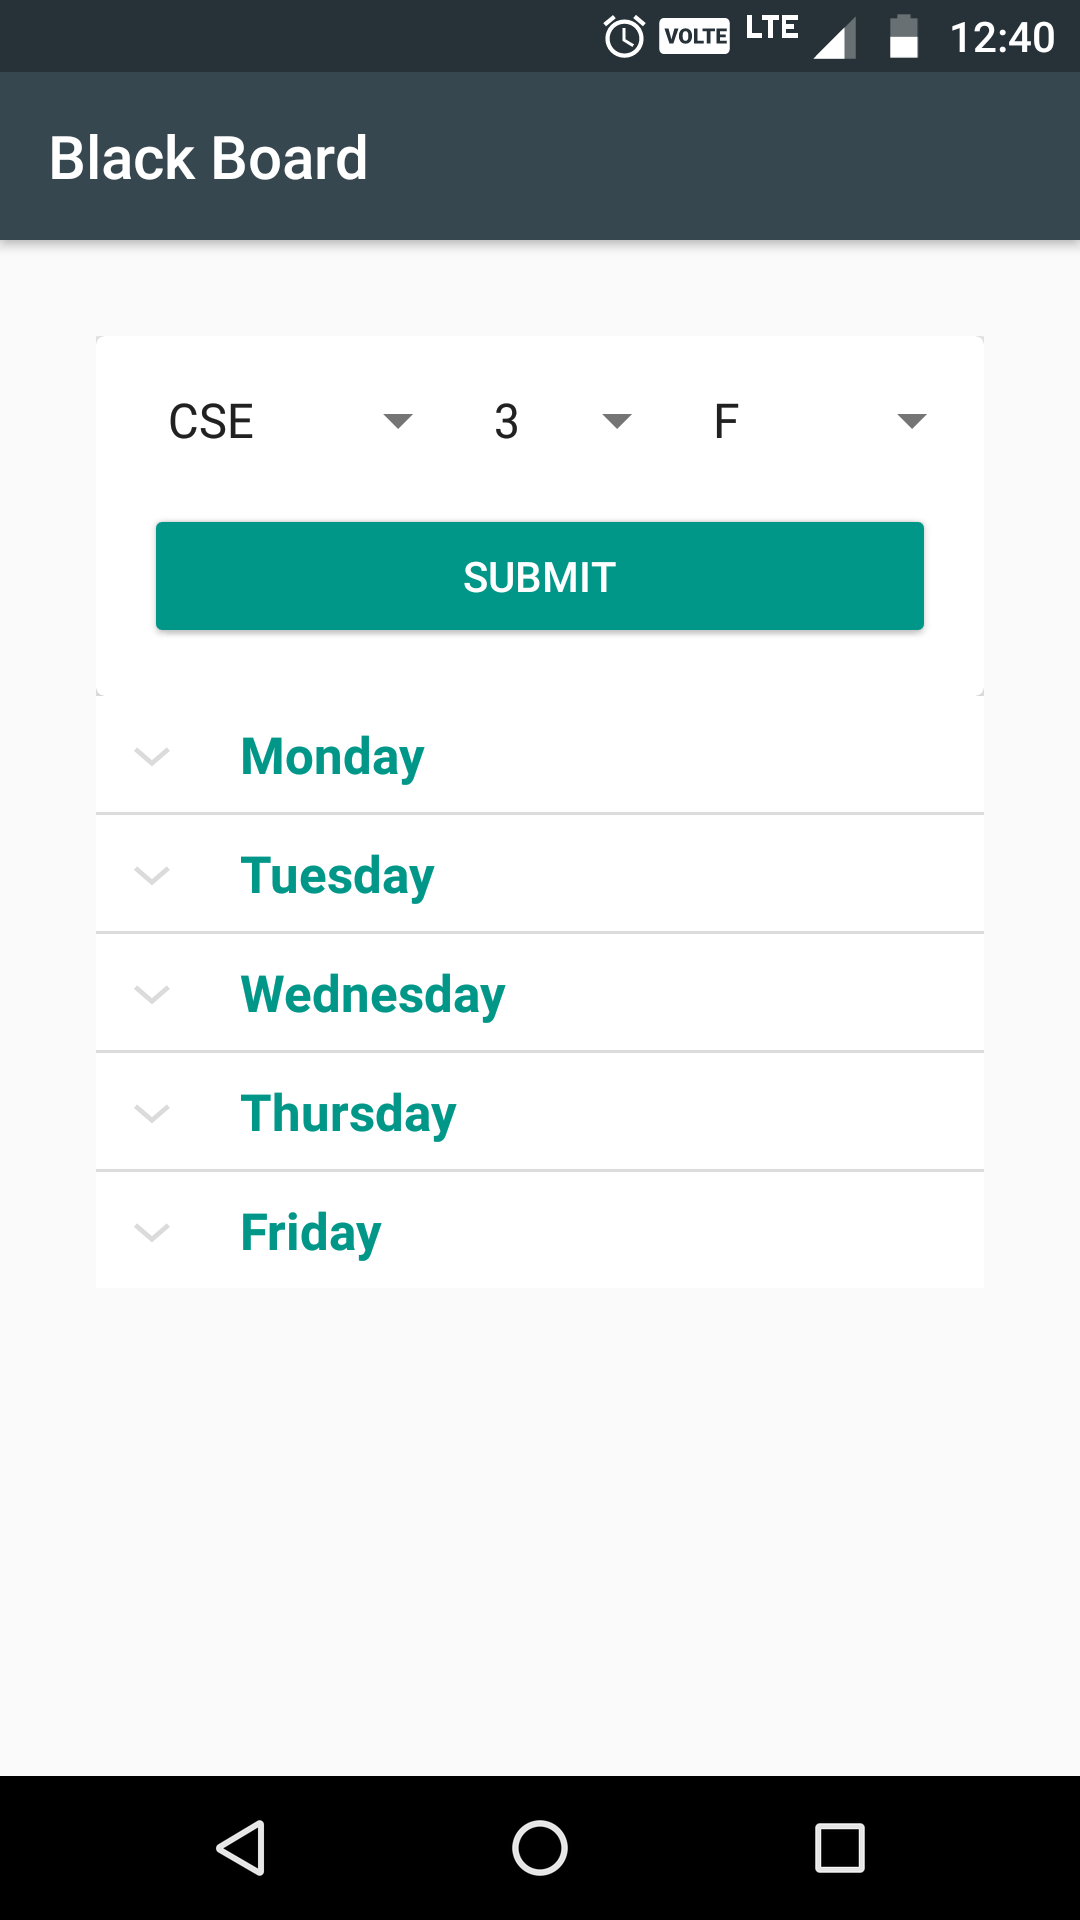
\includegraphics[width=\linewidth, height=7cm,keepaspectratio]{classtimetable}
\caption{Class Timetable}
\label{fig:class-timetable}
\end{figure} 
\subsubsection{Class Location (fig\ref{fig:class-location})}
The faculty can check the location of a particular class by selecting the dept, year, section of the class
\begin{figure}[htbp]
	\centering
	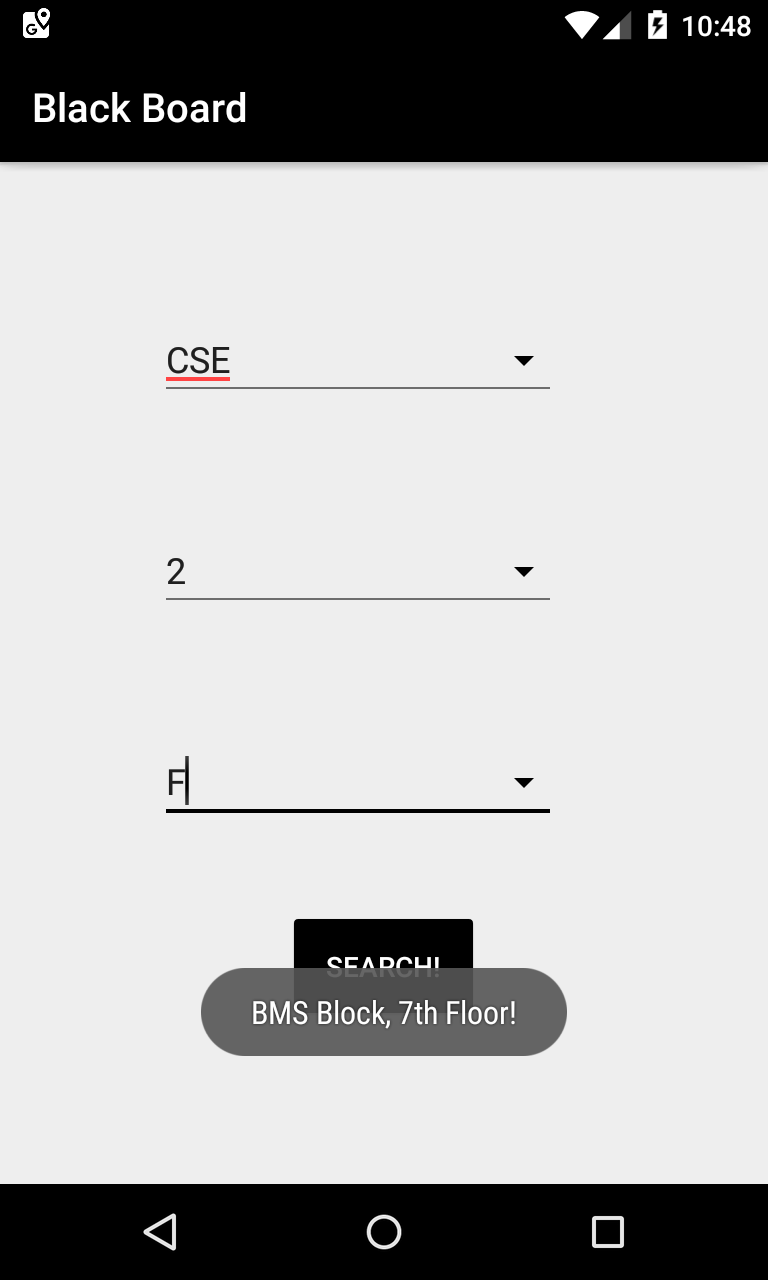
\includegraphics[width=\linewidth, height=7cm,keepaspectratio]{classlocation}
\caption{Class Location}
\label{fig:class-location}
\end{figure} 	
\subsubsection{Admin Login (fig\ref{fig:django-login})}
Login page for the Webportal where admin can login to change data.
\begin{figure}[htbp]
	\centering
	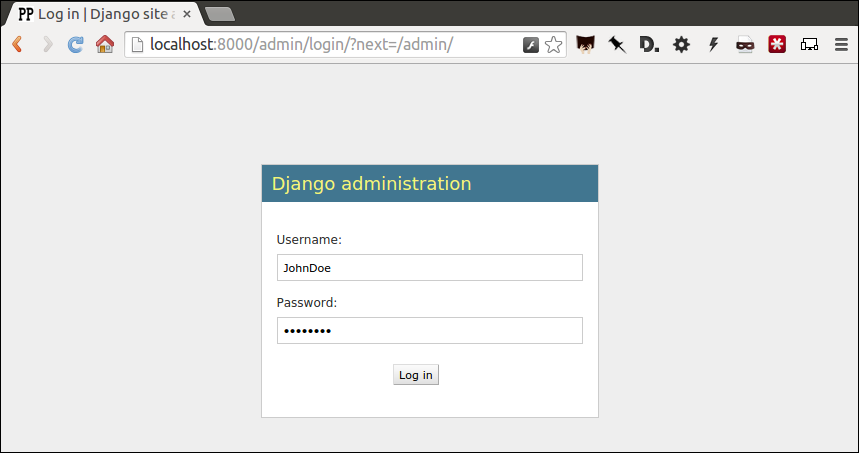
\includegraphics[width=\linewidth, height=7cm,keepaspectratio]{djangologin}
	\caption{BlackBoard Admin Login}
	\label{fig:django-login}
\end{figure} 
\subsubsection{Admin Dashboard (fig\ref{fig:django-dash})}
Dashboard for the admin Webportal where database can be modified/updated/added/deleted.
\begin{figure}[htbp]
	\centering
	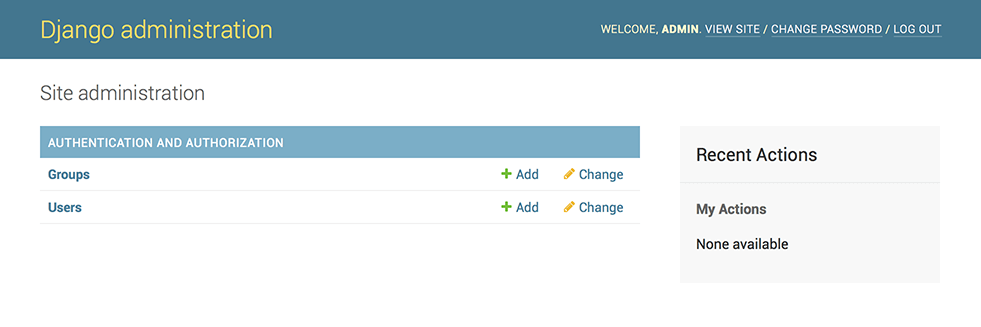
\includegraphics[width=\linewidth, height=7cm,keepaspectratio]{djangomanage}
	\caption{BlackBoard Admin Dashboard}
	\label{fig:django-dash}
\end{figure}
\begin{figure}[htbp]
	\centering
	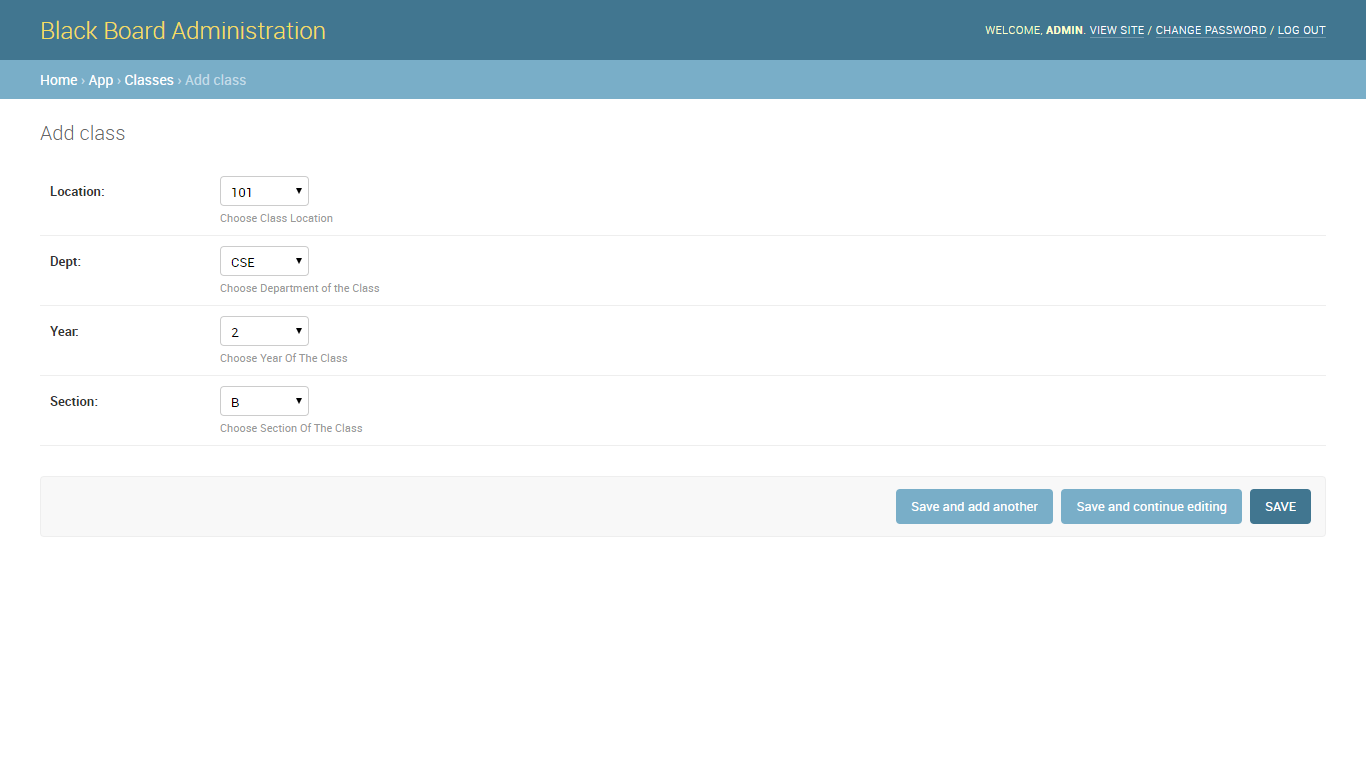
\includegraphics[width=\linewidth, height=7cm,keepaspectratio]{addclass}
	\caption{BlackBoard Admin- Add Class}
	\label{fig:django-dash}
\end{figure}
\begin{figure}[htbp]
	\centering
	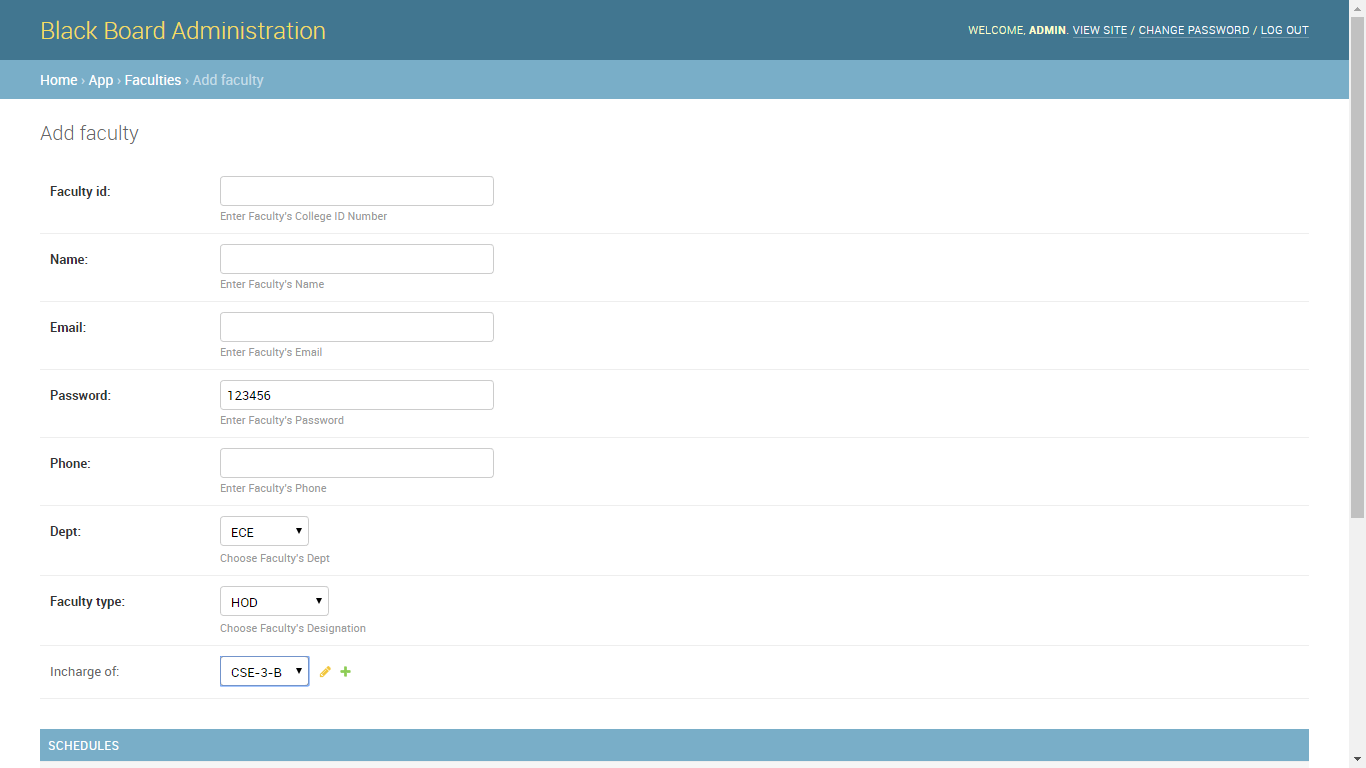
\includegraphics[width=\linewidth, height=7cm,keepaspectratio]{addfaculty}
	\caption{BlackBoard Admin-Add Faculty}
	\label{fig:django-dash}
\end{figure}
\begin{figure}[htbp]
	\centering
	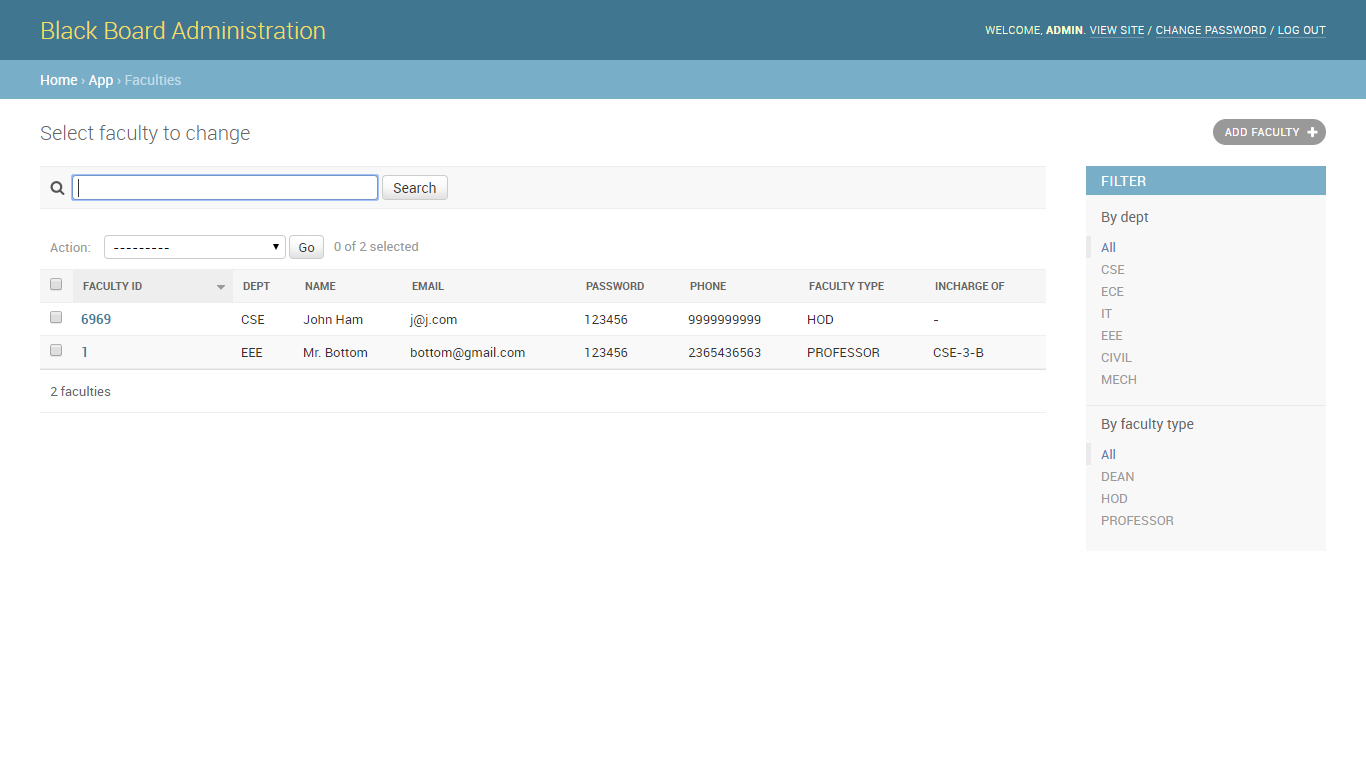
\includegraphics[width=\linewidth, height=7cm,keepaspectratio]{facultylist}
	\caption{BlackBoard Admin-faculty list}
	\label{fig:django-dash}
\end{figure}
\section{Summary}
The mobile application, incorporating the college
management system, is a very effective tool
which can be used for improving the overall efficiency in a college/university.During these tests, the number of arguments are compared to input parameters, matching of parameters and arguments etc.

The Application was tested on an emulator which lets you prototype, develop and test Android applications without using a physical device. The application performed extremely well in low resource environments where the storage space and network connection is slow. Memory leaks were detected and resolved during development using Leak Canary, Proguard has been used to optimize the code(remove unused resources) and also to obfuscate the core logic for security.


\chapter{Conclusion and future enhancement}
\section{Conclusion}
The mobile application, incorporating the college manage-
ment system, is a very effective tool which can be used

for improving the overall efficiency in a college/university.
The proposed mobile application portability and ease in use
increases its credibility compared to other state-of-art methods.
\section{Future Enhancement}
We plan to add another log-in for students where they can share documents related to subjects and also view their marks, attendance and all relevant information. This is only currently being implemented for our college. In the future, we plan to take it to various other colleges and institutions

% Bibliography.
\begin{singlespace}
\bibliography{biblo} % Enter your .bib file name here
\end{singlespace}
%%%%%%%%%%%%%%%%%%%%%%%%%%%%%%%%%%%%%%%%%%%%%%%%%%%%%%%%%%%%
\end{document}
